%%% Simulering for optimering af Current-sense filter %%%

\subsection{Current-sense filter}
Simuleringen af current-sense filteret sker ved, at måle current-sense signalet både før og efter filteret. Figur~\ref{fig:Simulering_PWM_current_sense_U_3} viser det ufiltrerede signal. Her ses stadig de forventede switching-spikes. Figur~\ref{fig:Simulering_PWM_current_sense_M_3} viser det filtrerede signal. Her aflæses stigetiden til ca. $85ns$, og derfor en hurtigere stigetid end det analyserede. Den hurtigere stigetid godtages, da switching-spikes'ene stadig er blevet filtreret væk. Det ses dog, at der kommer et lille overshoot på signalet. Det betyder at filterets stigetid kun lige præcis er lang nok til, at filtrere spikes'ene, men det er samtidig også denne balancegang, der er designet efter. 

\begin{figure}[H]
	\center
	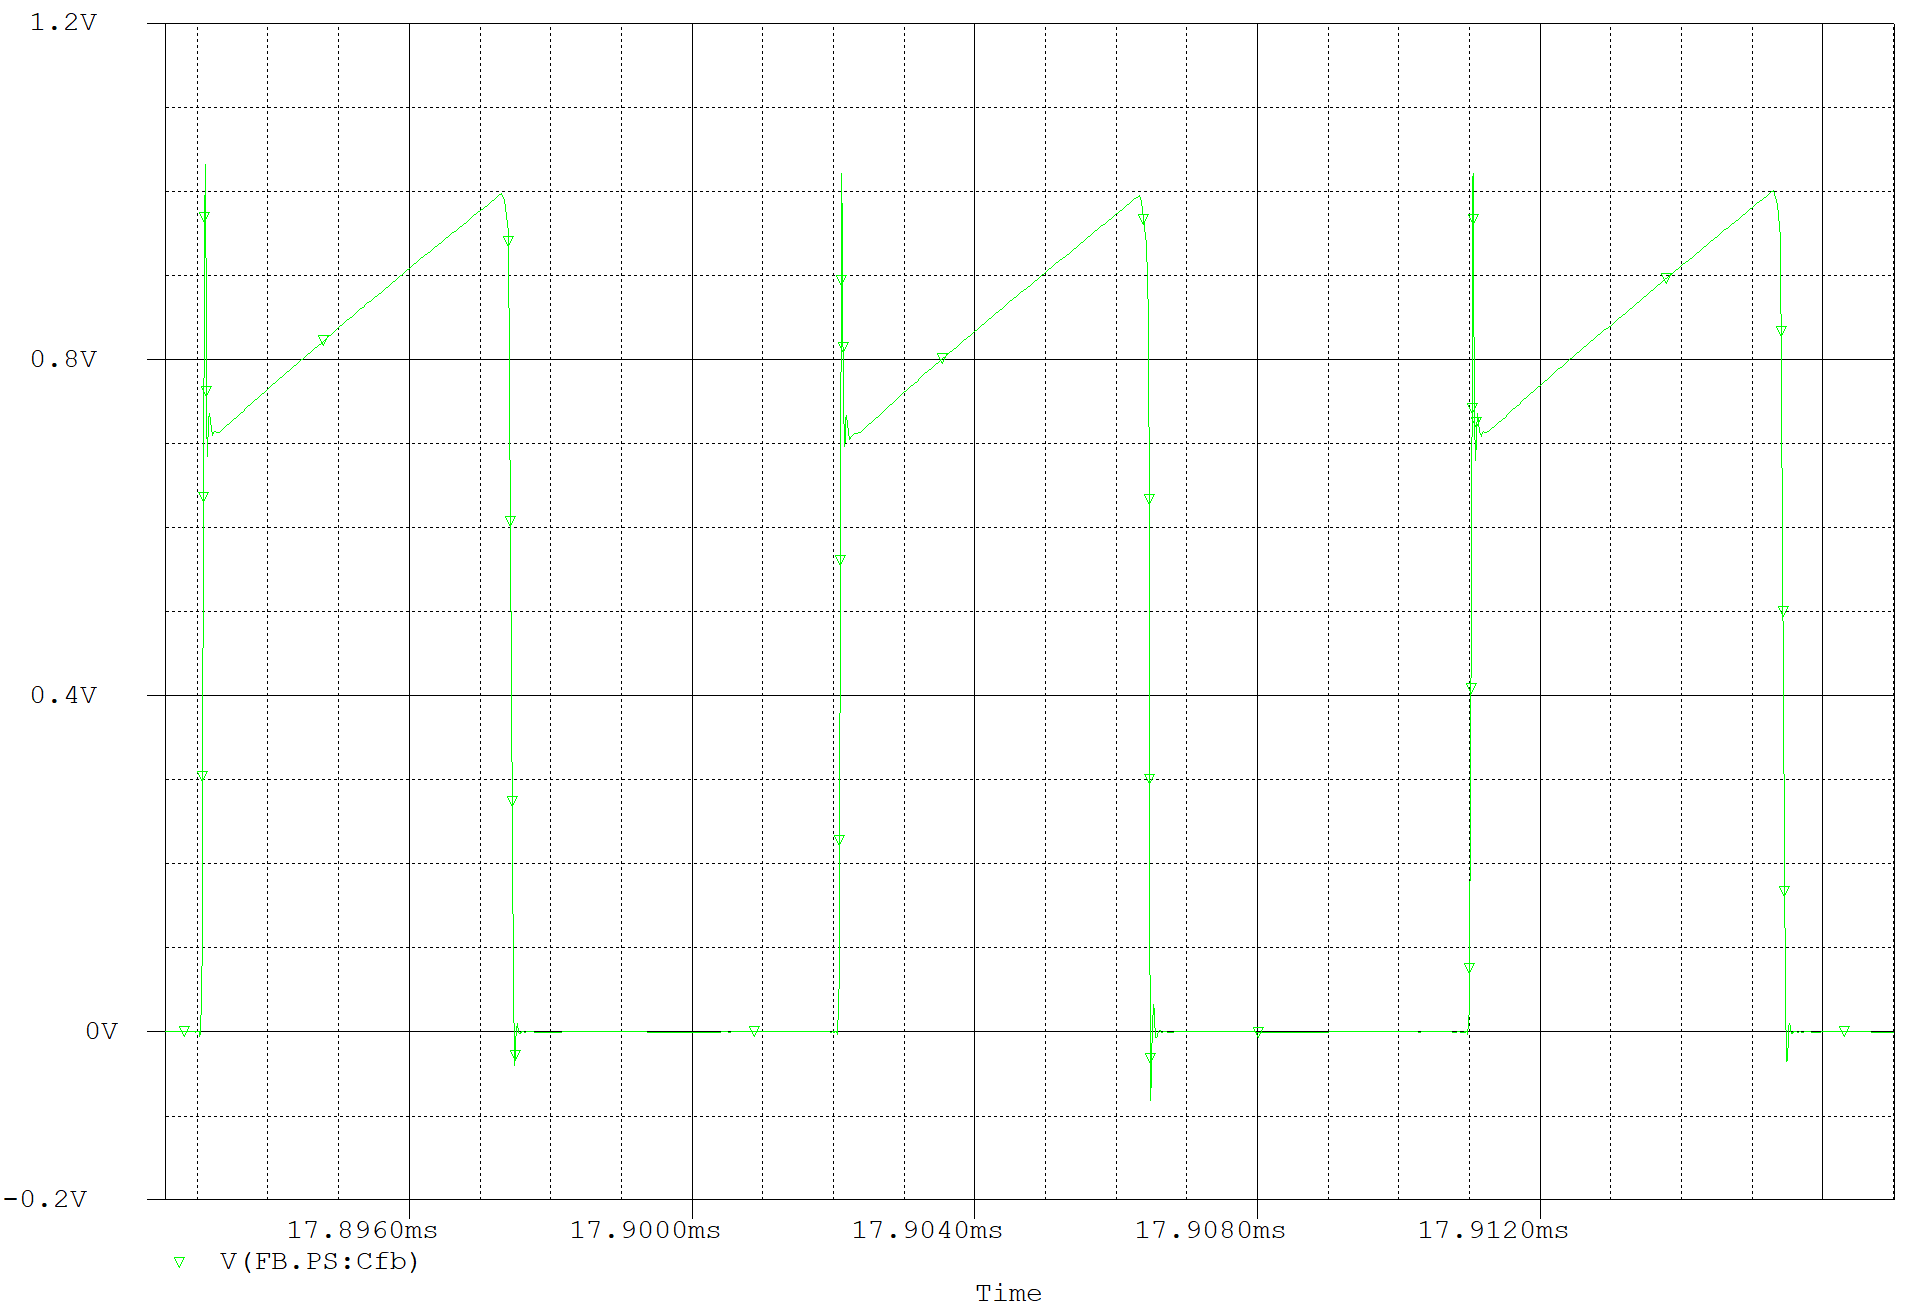
\includegraphics[max width=0.7\linewidth]{/tex/3iteration/billeder/Simulering/Simulering_cs_filter_U.png}
	\caption{Simulering af current-sense signal før filtrering}
	\label{fig:Simulering_PWM_current_sense_U_3}
\end{figure}

\begin{figure}[H]
	\center
	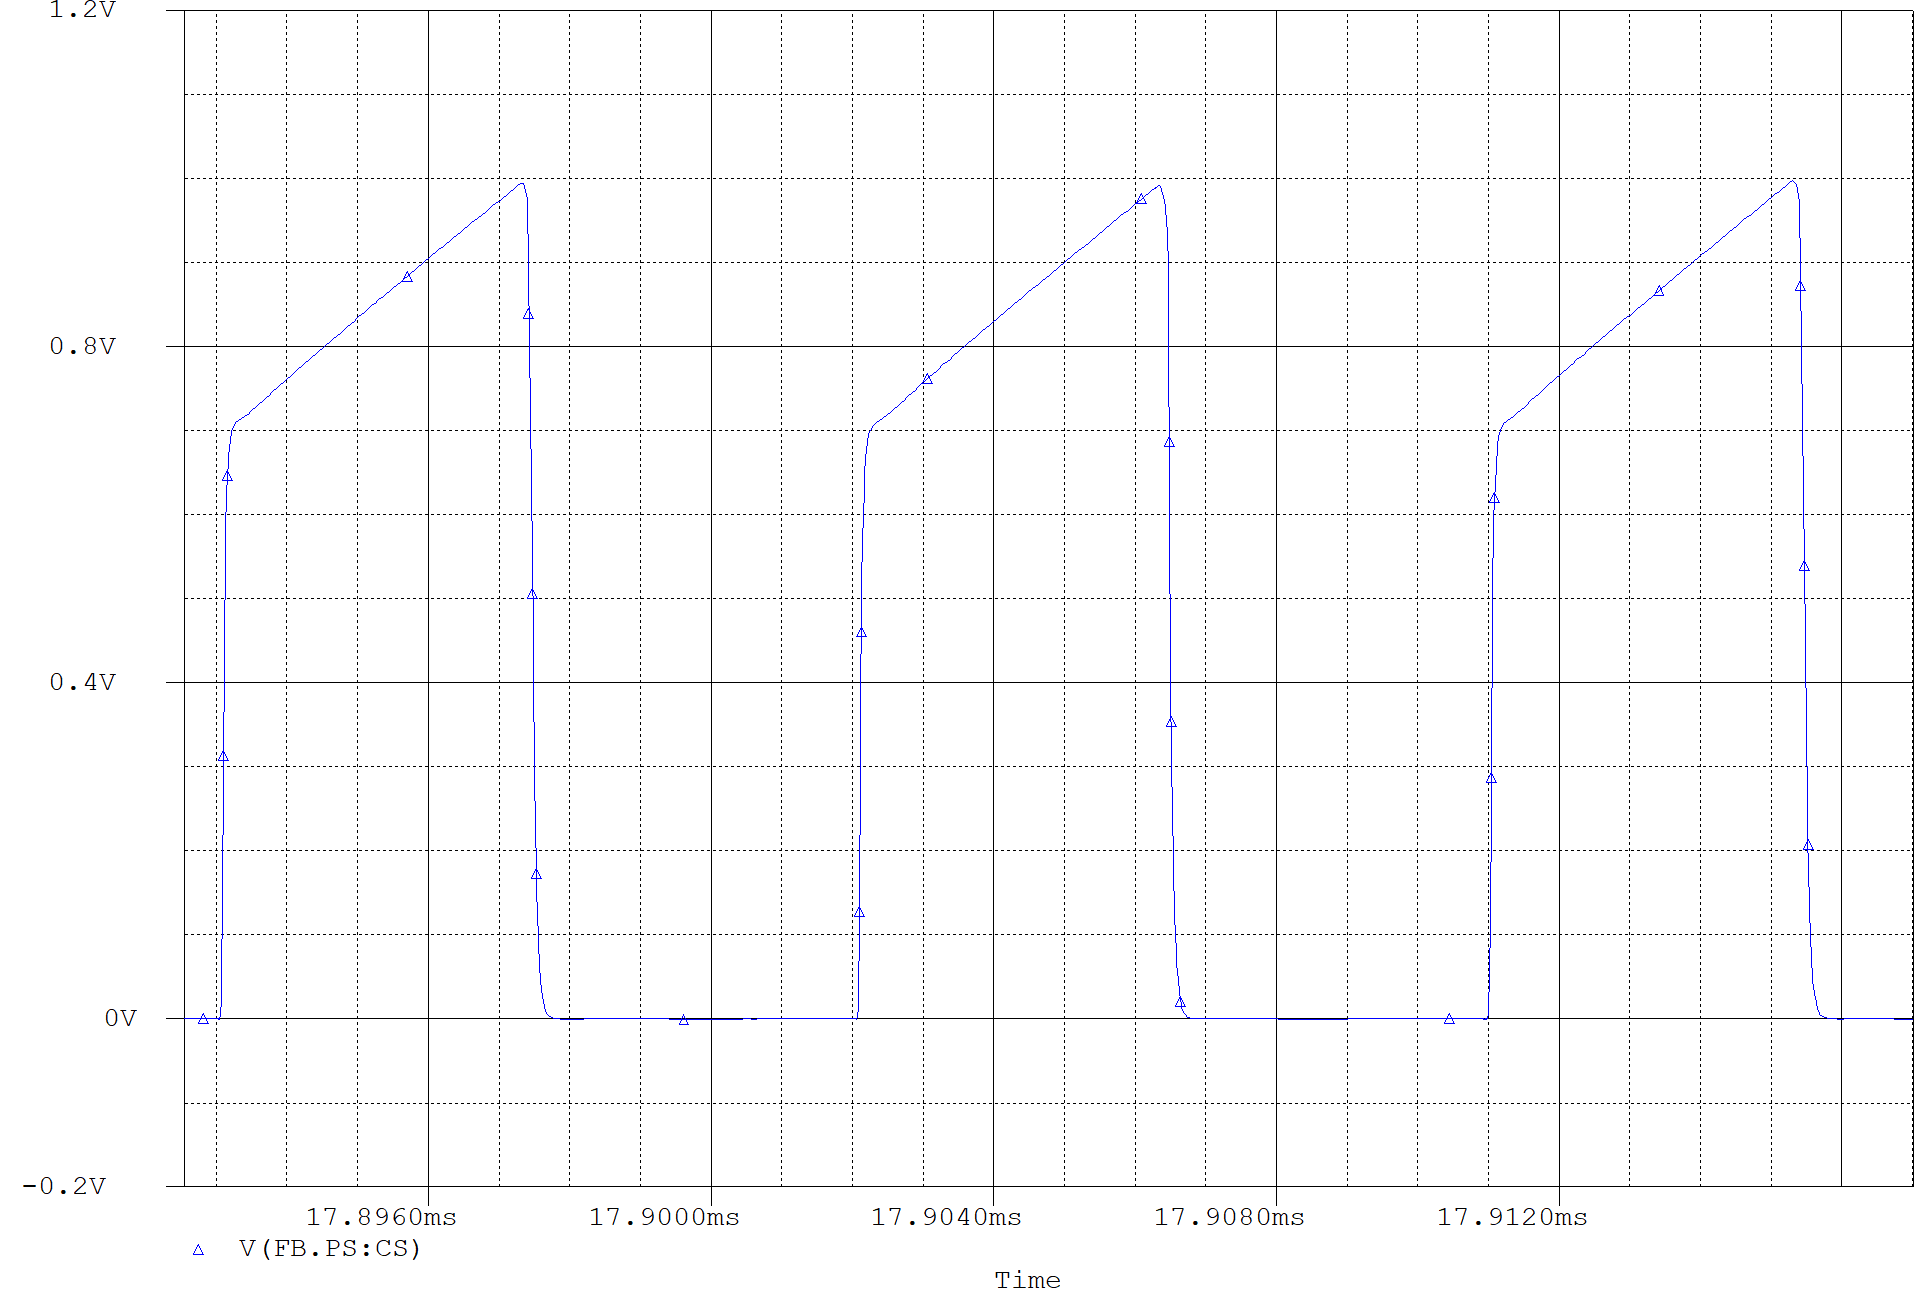
\includegraphics[max width=0.7\linewidth]{/tex/3iteration/billeder/Simulering/Simulering_cs_filter_M.png}
	\caption{Simulering af current-sense signal efter filtrering}
	\label{fig:Simulering_PWM_current_sense_M_3}
\end{figure}